\documentclass[useAMS,usenatbib]{mn2e}
\pdfoutput=1
\usepackage[varg]{txfonts}
\usepackage{astrojournals}
\usepackage{graphicx}
\usepackage{microtype}
\usepackage{xcolor}
\usepackage{fixltx2e}
\usepackage{hyperref}
\usepackage{siunitx}
\hypersetup{colorlinks=True, linkcolor=blue!50!black, citecolor=black,
  urlcolor=blue!50!black}

\usepackage[greek,english]{babel} 
\newcommand{\texttheta}{\greektext j\latintext}
\newcommand\thC{\texttheta\textsuperscript{1}\,Ori~C}
\newcommand\elec{\ensuremath{_{\mathrm{e}}}}
\newcommand\Ion[2]{\ensuremath{\mathrm{#1\,\scriptstyle #2}}}
\newcounter{ionstage}
\newcommand{\ion}[2]{% needs to be renewcommand with aastex
  \setcounter{ionstage}{#2}%
  \Ion{#1}{\Roman{ionstage}}}
\newcommand\nii{\ion{N}{2}}
\newcommand\sii{\ion{S}{2}}
\newcommand\oiii{\ion{O}{3}}

\begin{document}

%% Skip over the parts that are already written
\addtocounter{section}{6}
\addtocounter{subsection}{2}
\addtocounter{table}{5}
\addtocounter{figure}{9}


\subsection{A physical model of 177-341}
As an alternative to the purely empirical analysis presented in the previous sections, a different approach to analysing the emission spectrum of the proplyds is through the construction of physical models that combine a priori simulations of radiative transfer, hydrodynamics, and atomic physics in order to predict the density, temperature, and ionization structure of the proplyd flow.  
Such models have previously been applied to the ensemble properties of large numbers of proplyds \citep*{1998ApJ...499..758J, 1998AJ....116..322H} and in detail to individual objects such as 177-341 \citep{1999AJ....118.2350H}, LV2 \citep{2002ApJ...566..315H}, and LV1 \citep{2002ApJ...570..222G}. 
We have improved on these models in two significant ways.
First, whereas published models have considered only emission from regions where hydrogen is fully ionized and the flow is supersonic, we now use a detailed analytic model of gas acceleration in the ionization front \citep{2005ApJ...621..328H} to extend the treatment to cover partially ionized emission zones where the gas moves subsonically. 
Second, whereas published models used ad hoc fitting functions to the emissivity structure, specifically tailored to only the brightest emission lines, we now use the plasma micropysics code Cloudy \citep{1998PASP..110..761F} to self-consistently calculate the full physical structure and emission spectrum of the proplyd flow. 

\begin{table}
  \centering
  \caption{Input parameters for example physical model of 177-341} 
  \begin{tabular}{@{\,}ll@{\,}}\hline
    Stellar spectrum:& 
    \(T_* = \SI{39000}{K}\)\\
    \citep{2006AandA...448..351S} & \(\log g = 4.1\)\\
    & \(L_* = \num{2.04e5}\,L_\odot\)\\
    Ionizing flux at proplyd:& 
    \(\Phi_{\mathrm{H}} = \SI{1.58e13}{cm^{-2} s^{-1}}\)
    \\
    Ionization front radius:& 
    \(r_0 = \SI{1.91e15}{cm}\)
    \\
    Gas-phase abundances: & 
    He 10.98, C 8.41, N 7.85, O 8.30, \\
    (\(12 + \log_{10} z/\mathrm{H}\)) & Ne 7.56, S 6.98, Ar 6.26, Fe 5.65
    % Orion Nebula  \citep{2004MNRAS.355..229E}
    \\
    Dust composition: & Standard Orion \citep{1991ApJ...374..580B}\\
    \hline
  \end{tabular}
  \label{tab:model:pars}
\end{table}

\begin{figure*}
  \centering
  \begin{tabular*}{\linewidth}{@{\extracolsep{\fill}} ll}
    (\textit{a}) & (\textit{b}) \\
    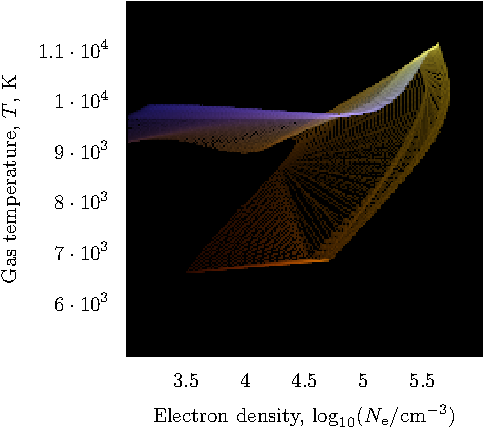
\includegraphics[width=0.45\linewidth]{NT-plane-SNO-RGB} &
    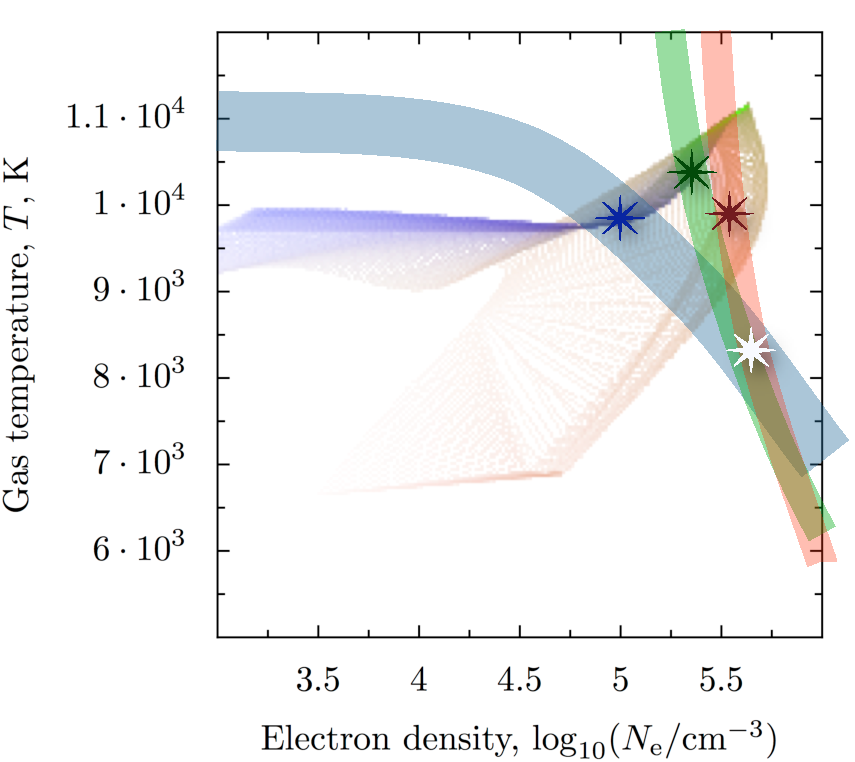
\includegraphics[width=0.465\linewidth]{ne-Te-overlay}
  \end{tabular*}
  \caption[]{Emission structure in the \(n\elec\)--\(T\elec\) plane for the example physical model of 177-341.  
    (\textit{a})~Positive-colored image of the three emission lines: [\sii] \SI{6731}{\AA} (red), [\nii] \SI{6584}{\AA} (green), and [\oiii] \SI{5007}{\AA} (blue), with brightness proportional to the fraction of the model luminosity in each line that comes from gas with that particular combination of density and temperature.  
The variations in density and temperature within the model are principally a function of radius within the proplyd, with a secondary variation as a function of angle between the ``nose'' and the ``ears'' of the proplyd crescent due to the increasing obliqueness of the illumination angle.  
The outer zones of the model are at low density and are highly ionized, emitting principally in [\oiii], as seen in the blue horizontal branch at \(\simeq \SI{9700}{K}\) in the upper left part of the figure.  
As one approaches the proplyd ionization front (direction of increasing density), the [\nii] and then [\sii] emission become relatively stronger (color changes to yellow) and the temperature increases, reaching a maximum of \(\simeq \SI{11000}{K}\).  
In the ionization front itself, the temperature drops while the electron density climbs to a peak of about \SI{3e5}{cm^{-3}} and then also falls.  At the same time, the [\sii] emission comes to dominate over [\nii], giving rise to the orange-red branch that curves down and to the left.  
(\textit{b})~Negative-colored image of the same data as in \textit{a} overlayed with the observational diagnostic curves from Fig.~7\textit{a} ([\sii] in red, [\nii] in green, [\oiii] in blue).  
The white star shows the solution for \(n\elec, T\elec\) obtained in \S~4.2 under the assumption that the emission in all three ions is co-extensive at a single density and temperature.   
This solution lies well outside the locus of densities and temperatures seen in the model, even though the model \emph{does} reproduce the observed line ratios. 
Instead, the model satisfies the constraints of the three diagnostic curves separately in three different regions, which are indicated schematically by the colored stars.  
Note, however that even within the emission region of each ion there is considerable variation in the physical conditions.  
}
  \label{fig:model:nT}
\end{figure*}

\begin{figure*}
  \centering
  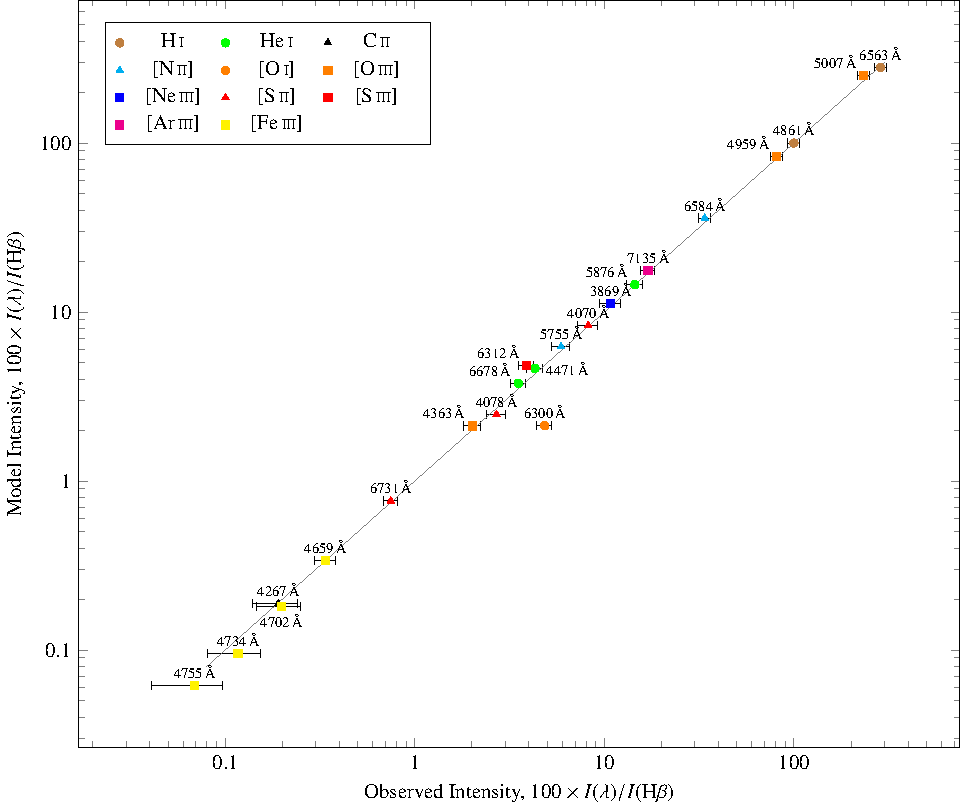
\includegraphics[width=\linewidth]{ratios-figure-figure10}
  \caption{Comparison of model and observed line intensities for the proplyd 177-341.  The model parameters are those given in Table~\ref{tab:model:pars} and the emission structure of the model is discussed in Fig.~\ref{fig:model:nT}.   
Observed intensities correspond to the \(c(\mathrm{H}\beta) = 0\) background-subtracted values given in column~4 of Table~2.
  }
  \label{fig:model}
\end{figure*}


Preliminary results of the emission line spectrum of such a model applied to 177-341 are shown in Figures~\ref{fig:model:nT} and \ref{fig:model}.  
The input parameters for the model (values given in Table~\ref{tab:model:pars}) are the radius of the ionization front at the proplyd cusp (assumed hemispherical), the intensity and spectral shape of the illuminating stellar radiation, and the composition (gas-phase elemental mix and dust grain populations) of the proplyd material.
For most of these parameters, we have taken values from the literature, whereas the gas-phase abundances and incident ionizing flux have been adjusted slightly in an attempt to reproduce the observed emission line intensities. 
The stellar spectrum is that determined for the ionizing star \thC{} by spectroscopic analysis \citep{2006AandA...448..351S}. 
The ionization front radius is the value determined by fitting to \textit{HST} emission line images \citep{1999AJ....118.2350H}, while the adopted ionizing flux at the proplyd position corresponds to a physical separation of the proplyd from the ionizing star of \SI{2.13e17}{cm} if there is no intervening absorption.
Given the observed angular separation of \(25.84''\) \citep{1998AJ....116..293B}, and assuming a distance to the Orion Nebula of 440~pc (\citealp{2008AJ....136.1566O}, Appendix~A), the projected separation is \SI{1.70e17}{cm}, implying an inclination angle of \(\simeq 55^\circ\). 
The diffuse radiation field and the proplyd tail are ignored in this model, since the observational aperture (\S~2.2) only covers the head of the proplyd. 

Figure~\ref{fig:model} shows that the model generally reproduces very well the observed relative line intensities for 177-341 with the notable exception of the [\ion{O}{1}] \SI{6300}{\AA} line, which has a predicted intensity of only half the observed value.
This discrepancy may be explained if a significant fraction of the observed [\ion{O}{1}] emission comes from dissociation of OH at the surface of the proplyd's circumstellar disk \citep{1998ApJ...502L..71S}, which is not included in our model.
The only other disagreement is with the [\ion{S}{3}] \SI{6312}{\AA} line, which is roughly 25\% too high in the model (roughly 1.5 times the observational uncertainty). 
This may be an indication that the details of the stellar spectrum around \SI{23}{eV} are not correctly modeled, although the disagreement is only marginal. 

Given that the stellar spectrum is very well constrained, the only way to vary the model temperature by a significant amount is by changing the gas-phase metal abundances and thus the gas cooling rate.  
In particular, the temperature in the highly ionized outer regions of the proplyd is very sensitive to the oxygen abundance since the [\oiii] \SI{5007}{\AA} line is the major coolant there. 
In order to reproduce the observed line intensities (particularly the [\oiii] \SI{4363}{\AA}/\SI{5007}{\AA} ratio), we find it necessary to reduce the oxygen abundance to less than 50\% of the value that has been measured for the surrounding nebula (e.g., \citealp{2004MNRAS.355..229E}), which leads to a temperature of around \SI{9500}{K} in the [\ion{O}{3}] emission zone. 
Using the standard Orion gas-phase abundances gives temperatures of about \SI{8500}{K} for the same zone and predicts [\ion{O}{3}]/H\(\beta\) ratios that are considerably higher than observed for the nebular \SI{5007}{\AA} and \SI{4959}{\AA} lines, but lower than observed for the auroral \SI{4363}{\AA} line. 
Using the even higher abundances derived by \citet{Tsamis:2011} for the proplyd LV2 implies temperatures as low as \SI{7700}{K} and exacerbates the disagreement with the observations still further. 
For comparison, both varying the stellar effective temperature by \(\pm \SI{1000}{K}\) (the uncertainty in the analysis of \citealp{2006AandA...448..351S}) or varying the ionizing flux by a factor of two (corresponding to the uncertainty in the inclination angle of the proplyd) only change the gas temperature by \(<\SI{200}{K}\), while varying the stellar atmosphere model between WMBasic \citep{2001A&A...375..161P} and TLUSTY \citep{2003ApJS..146..417L} produces a slightly larger change of \(\simeq \SI{400}{K}\).  

Despite the promising success of the model in reproducing the observed line intensities, further work is necessary before a definitive statement can be made about the gas-phase abundances in the proplyd.  
The lack of observations of [\ion{O}{2}] lines, together with the uncertain nature of the [\ion{O}{1}] emission (see above) means that the oxygen abundance hinges on observations of a single ion stage.  
It is vital to test the model against other proplyds, particularly those such as LV2 \citep{Tsamis:2011, Tsamis:2011a} where the [\ion{O}{2}] \num{3726}, \SI{3729}{\AA} doublet is observed.  
At the same time, the models need to be simultaneously constrained not just by the line ratios, but also by sub-arcsecond \textit{HST} imaging \citep{1998AJ....116..293B, 1998AJ....115..263O} and velocity profiles from high-resolution spectroscopy \citep{1999AJ....118.2350H, Shuping:2003a}. 
It is also necessary to examine in greater detail the potential influence of internal extinction within the proplyd. 
This depends on the properties of the dust that is entrained in the photoevaporation flow, which can be constrained by comparison with observations of thermal mid-infrared emission \citep{2001ApJ...561..830G, Smith:2005, 2005AJ....129.1534R, Shuping:2006}.



\section*{Acknowledgements}

WJH and NFF acknowledge financial support from DGAPA-UNAM through project PAPIIT IN102012 and from a postdoctoral fellowship to NFF\@. 


\bibliographystyle{mn2e}
\bibliography{BibdeskLibrary}

\end{document}
